\chapter{Bóg szabatu a Bóg niedzieli — J. B. Frisbie}

Istnieją inne artykuły na temat \emcap{osobowości Boga} napisane przez naszych pionierów i trudno byłoby zawrzeć tu wszystkie, ale chcielibyśmy dodać jeszcze jedno świadectwo z artykułu brata J. B. Frisbie’go, w którym porównuje on Boga szabatu z Bogiem niedzieli. Porównuje on prawdę o \emcap{osobowości Boga} wyrażoną w pierwszym punkcie \emcap{Fundamentalnych Zasad} z doktryną o Trójcy. Przyjrzyjmy się fragmentowi jego artykułu „\textit{Szabat dnia siódmego nie zniesiony}” z \textit{Review and Herald} z 7 marca 1854 roku.

\begin{figure}[hp]
    \centering
    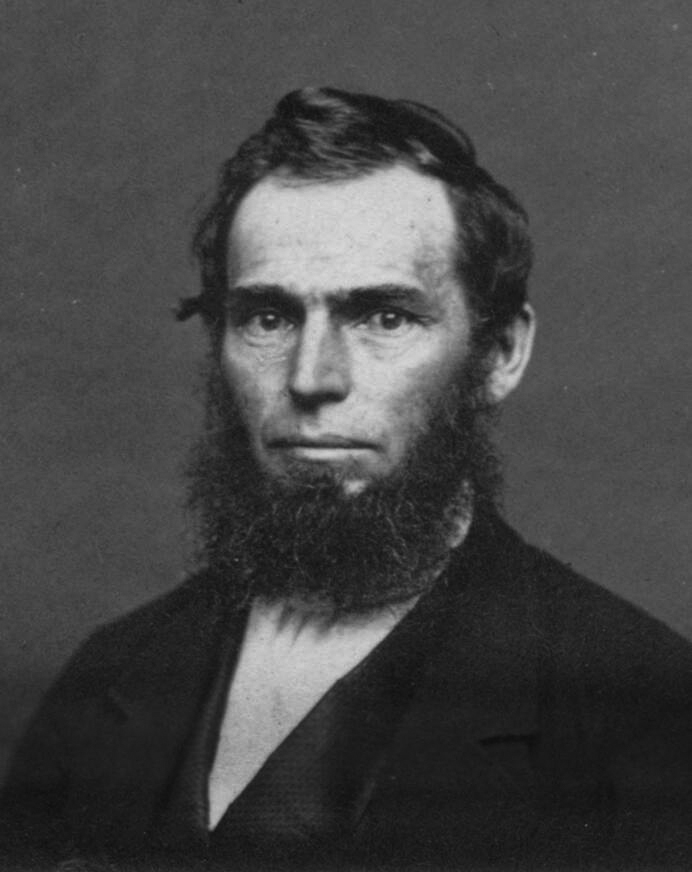
\includegraphics[width=1\linewidth]{images/j-b-frisbie.jpg}
    \caption*{John Byington Frisbie (1816-1882)}
    \label{fig:j-b-frisbie}
\end{figure}


\section*{Bóg szabatu}

\others{Gdy poznamy Boga i będziemy o Nim pamiętać, przestrzegając Jego świętego szabatu, \textbf{wtedy Biblia nauczy nas o Jego osobowości i miejscu zamieszkania}. \textbf{Człowiek jest na obraz i podobieństwo Boga}. Rdz 1:26. «I rzekł Bóg: Uczyńmy (mówiąc do swojego syna) człowieka na nasz obraz, według naszego podobieństwa». Rozdz. 2:7. «I ukształtował Pan Bóg człowieka z prochu ziemi, i tchnął w jego nozdrza tchnienie życia. I stał się człowiek duszą żyjącą». Rdz 9:6; 1Kor 11:7; Jk 3:9. \textbf{To, co zostało stworzone na \underline{obraz i podobieństwo Boga}, zostało uczynione z prochu ziemi i nazwane człowiekiem}.}

\othersnogap{To jest uznawane za prawdziwe znaczenie na podstawie innych świadectw, które można znaleźć w Biblii. \textbf{Jezus był w postaci człowieka i dokładnym obrazem osoby swojego Ojca}.}

\othersnogap{Flp 2:6--8. \textbf{Chrystus Jezus}: «Który, będąc w \textbf{postaci Boga}, nie uważał za grabież być \textbf{równym Bogu}. Lecz ogołocił samego siebie i przyjął \textbf{postać sługi}, i \textbf{został uczyniony na podobieństwo ludzi}». 2Kor 4:4. \textbf{«A będąc ukształtowany na wzór człowieka»}... Kol 1:15. «\textbf{Który jest obrazem niewidzialnego Boga}».}

\othersnogap{Hbr 1:3. \textbf{Syn; «Który, będąc jasnością jego chwały i dokładnym obrazem jego osoby»}. W tym sensie Jezus mógł zgodnie z prawdą powiedzieć do Filipa: «Kto mnie widział, widział i Ojca». J 14:9. Niektórzy wydają się sądzić, że \textbf{przeczy to osobowości Boga, \underline{ponieważ jest On Duchem, i mówią, że nie ma On ciała ani części ciała}}. J 4:24. «\textbf{Bóg jest duchem}». Hbr 1:7. «\textbf{Który czyni swoich aniołów duchami}». \textbf{Kto ośmieliłby się twierdzić, że aniołowie nie mają ciał ani części ciała, ponieważ są duchami}? \textbf{\underline{Niemniej jednak Bóg jest istotą duchową posiadającą ciało i części ciała, o czym dowiadujemy się przez to, że ma miejsce zamieszkania, i ponieważ można go zobaczyć}}. Wj 33:23. «I odejmę moją rękę, i \textbf{ujrzysz moje plecy}, ale \textbf{moje oblicze nie będzie widziane}». Mt 5:8. «Błogosławieni czystego serca, albowiem \textbf{oni zobaczą Boga}». Hbr 12:14. «Dążcie do pokoju ze wszystkimi i do świętości, bez której \textbf{nikt nie ujrzy Pana}». Mt 18:10. «Że w niebie ich aniołowie \textbf{zawsze patrzą na oblicze mojego Ojca, który jest w niebie}». Mt 6:9. «Wy więc tak się módlcie: \textbf{Ojcze nasz, który jesteś w niebie}»... J 6:38. «Bo \textbf{zstąpiłem z nieba} nie po to, żeby czynić swoją wolę, lecz wolę tego, który mnie posłał». Rozdz. 16:28. «\textbf{Wyszedłem od Ojca i przyszedłem na świat}; znowu \textbf{opuszczam świat i idę do Ojca}».}

\othersnogap{\textbf{Czy Bóg nie mówi, że wypełnia nieskończoność przestrzeni? \underline{Odpowiadamy: Nie}}. Ps 139:7, 8. «Dokąd ujdę przed \textbf{twoim duchem}? I dokąd ucieknę przed \textbf{twoją obecnością}? Jeśli wstąpię do nieba, ty tam jesteś»... \textbf{\underline{Bóg przez swojego Ducha może wypełniać niebo i ziemię}}. \textbf{Niektórzy mylą Boga z Jego Duchem, co prowadzi do zamieszania}. Ps 11:4. «\textbf{Pan jest w swoim świętym przybytku, tron Pana jest w niebie}: jego oczy patrzą...». Ha 2:20; Ps 102:19. «Bo spojrzał \textbf{w dół z wysokości swojej świątyni}; \textbf{\underline{z nieba} Pan popatrzył na ziemię»}. 1P 3:12. «Oczy Pana są nad sprawiedliwymi, a jego uszy otwarte są na ich modlitwy...». Ps 80:1. ‘Słuchaj, Pasterzu Izraela, ty, który prowadzisz Józefa jak stado; ty, \textbf{który mieszkasz między cherubinami}, zajaśniej». Ps 99:1; Iz 37:16.}

\othersnogap{J 14:2. «W domu mego Ojca jest wiele posiadłości. Idę przygotować miejsce dla was». Obj 21:2--5; Hbr 11:6. «Bo kto przychodzi do Boga, musi wierzyć, że on jest...». \textbf{To świadectwo uważamy za niezwykle ważne w tym czasie, ażeby wiedzieć, iż jest Bóg. Nie mamy wątpliwości, że gdyby nasze oczy mogły zostać otwarte w wizji lub widzieć tak, jak widzą aniołowie, zobaczylibyśmy Boga w niebie siedzącego na swoim tronie, i jest On obecny we wszystkim, co istnieje, bez względu na to, jak daleko od Niego w Jego stworzeniu}.}[\href{https://documents.adventistarchives.org/Periodicals/RH/RH18540307-V05-07.pdf}{Adventist Review and Sabbath Herald, 7 marca 1854}, J. B. Frisbie, “The Seventh-Day Sabbath Not Abolished”, str. 50]

Tutaj widzimy ten sam argument i rozumowanie, że Bóg jest osobową istotą duchową. Ten Bóg jest Bogiem szabatu. Brat Frisbie porównuje tego Boga z Bogiem niedzieli, który jest Bogiem trynitarnym.

\section*{Bóg niedzieli}

\others{Przedstawimy kilka fragmentów, aby czytelnik mógł \textbf{zobaczyć wyraźny kontrast między \underline{Bogiem Biblii} ujawnionym na światło przez zachowywanie szabatu, a bogiem w ciemności przez zachowywanie niedzieli}. Skrócona wersja katechizmu Kościoła katolickiego autorstwa Wielebnego Johna Dubois, Biskupa Nowego Jorku. Strona 5. «\textbf{Pyt. Gdzie jest Bóg? Odp. Bóg jest wszędzie}. P. Czy Bóg widzi i wie wszystko? O. Tak, On wie i widzi wszystko. \textbf{P. Czy Bóg ma ciało? O. \underline{Nie; Bóg nie ma ciała, jest jedynie Duchem}}. \textbf{P. Czy jest więcej Bogów niż jeden? O. Nie; jest tylko jeden Bóg. P. Czy jest więcej osób niż jedna w Bogu? O. \underline{Tak; w Bogu są trzy osoby}. P. Które to są? O. Bóg Ojciec, Bóg Syn i Bóg Duch Święty. P. Czy nie ma trzech Bogów? O. Nie; Ojciec, Syn i Duch Święty to wszystko jeden i ten sam Bóg}».}

\othersnogap{Pierwszy artykuł Religii Metodystycznej, str. 8. \textbf{«Jest tylko jeden żywy i prawdziwy Bóg}, wieczny, \textbf{bez ciała i części ciała}, o nieskończonej mocy, mądrości i dobroci: stwórca i zachowawca wszystkich rzeczy, widzialnych i niewidzialnych. \textbf{A w jedności tego Bóstwa są trzy osoby jednej substancji, mocy i wieczności; Ojciec, Syn i Duch Święty}.’}

\othersnogap{W tym artykule, podobnie jak w doktrynie katolickiej, \textbf{uczy się nas, że są trzy osoby jednej substancji}, mocy i wieczności tworzące \textbf{w sumie jednego żywego i prawdziwego Boga}, wiecznego \textbf{bez ciała i części ciała}. Ale w tym wszystkim nie powiedziano nam, \textbf{co stało się z ciałem Jezusa, który miał ciało, gdy wstąpił do nieba, który poszedł do Boga, który ‘jest wszędzie» albo nigdzie}. Doksologia.}

\othersnogap{«\textbf{Bogu Ojcu, Bogu Synowi,}} \\
\others{\textbf{Trzem w jednym i Bogu Duchowi}».} \\
\others{Znowu} \\
\others{«Grzeje w słońcu, orzeźwia w powiewie,} \\
\others{Świeci w gwiazdach i kwitnie na drzewie.} \\
\others{\textbf{Wypełnia wszelkie życie, bezkres obejmuje},} \\
\others{Niesie się niepodzielnie i się nie wyczerpuje». — Papież.}

\othersnogap{Te idee dobrze współgrają z poglądami filozofów pogańskich. Jeden mówi, «że woda była podstawą wszystkich rzeczy, a Bóg jest tą duchową istotą, przez którą wszystkie rzeczy są kształtowane z wody». Inny, «że powietrze jest Bogiem, że jest wytwarzane, że jest niezmierzone i nieskończone...». Trzeci, «że Bóg jest duszą przenikającą wszystkie byty natury...». \textbf{Niektórzy wyznają ideę \underline{wyłącznie Ducha}}. I wreszcie, «że Bóg jest wieczną substancją».}

\othersnogap{Te fragmenty są wzięte z \textit{The Ancient History} autorstwa Rollina, tom II, str. 597--598, wydanej przez Harpers. \textbf{Nie powinniśmy raczej wierzyć, że bóg niedzieli pochodzi z tego samego źródła co zachowywanie niedzieli}. «Niedziela (Sunday) była nazwą nadaną przez pogan pierwszemu dniowi tygodnia, ponieważ był to dzień, w którym czcili słońce (the sun)». — The Union Bible Dictionary. \textbf{Później została zmodyfikowana przez Kościół rzymskokatolicki do postaci, w jakiej obecnie jest nauczana w całym kraju}.}

\othersnogap{Bardzo naturalne jest przypuszczenie, że gdy \textbf{Papież ustanowił się Bogiem w świątyni Bożej} [2Tes 2:4], musiał mieć dzień poświęcony dla swojej czci. To właśnie uczynił. — Douay, Katechizm, str. 59. «P. Jaki jest najlepszy sposób na uświęcenie niedzieli? O. Między innymi przez słuchanie mszy. To odprawianie mszy polega na tym, że ksiądz mamrocze po łacinie, pije wino i daje ludziom opłatek do zjedzenia».} \others{Ale Bóg uświęcił swój dzień, ponieważ w nim odpoczął. Inny dzień do zupełnie innego celu. Rdz 2:3.}

\othersnogap{W dniach przed moralnym upadkiem Babilonu Bóg zwracał umysły swoich szczerych dzieci we właściwym kierunku w ich modlitwach, bez względu na to, co mogłyby myśleć w innych chwilach, ale teraz od czasu odstępstwa umysł nie dociera do żadnego boga, tylko do ludzi, jest wiele modlitw do ludzi, które rozpoznajemy po ich wpływie i elokwencji. \textbf{Jesteśmy prawdziwie wdzięczni naszemu niebiańskiemu Ojcu, że \underline{wyprowadził nasze umysły z takiego szaleństwa}, abyśmy poznali i pamiętali \underline{Jego święte imię} przez zachowywanie Jego świętego dnia, abyśmy mogli Go kochać, służyć Mu i godnie \underline{Go chwalić przez naszego wielkiego Arcykapłana w niebiańskiej Świątyni w tym dniu pojednania}}.}[Tamże.][https://documents.adventistarchives.org/Periodicals/RH/RH18540307-V05-07.pdf]

Zanim został adwentystą dnia siódmego, Frisbie był kaznodzieją metodystycznym i zagorzałym przeciwnikiem wierzeń adwentystycznych. W 1853 roku, po debacie na temat szabatu z Josephem Batesem, zmienił swoje stanowisko i zaczął zachowywać szabat oraz głosić doktrynę Adwentystów Dnia Siódmego. Wyrzekł się niedzieli, Trójcy i przyjął prawdę o szabacie dnia siódmego oraz prawdę o Bogu, której Adwentyści Dnia Siódmego nauczali w pierwszym punkcie \emcap{Fundamentalnych Zasad}.

Czy inni pionierzy adwentyzmu dostrzegają niezgodność między doktryną o Trójcy a \emcap{osobowością Boga} wyrażoną w pierwszym punkcie \emcap{Fundamentalnych Zasad}?

% Bóg szabatu a Bóg niedzieli - J. B. Frisbie

\begin{titledpoem}

    \stanza{
        Dwa obrazy Boga, dwie różne natury, \\
        Jeden prawdą jaśnieje, drugi w cieniu bury. \\
        Bóg szabatu osobą z ciałem i częściami, \\
        Bóg niedzieli bezkształtny, rozlany nad światami.
    }

    \stanza{
        Na obraz Stwórcy człowiek uformowany, \\
        Z prochu ziemi przez Boga mądrze ukształtowany. \\
        Syn jest obrazem Ojca, doskonałym odbiciem, \\
        Kto widział Syna, Ojca ujrzał z zachwytem.
    }

    \stanza{
        Bóg ma tron w niebie, miejsce przebywania, \\
        Przez Ducha swego wszędzie jest od zarania. \\
        Nie jest On wszędzie obecny w swej istocie, \\
        Lecz przez Ducha działa w każdej życia dobrocie.
    }

\end{titledpoem}

\begin{titledpoem}

    \stanza{
        Szabat czy niedziela – więcej niż dzień tygodnia, \\
        To wyznanie wiary, co duszę rozpogadnia. \\
        Szabat wskazuje na Boga osobowego, \\
        Niedziela na bóstwo z pogaństwa wyjętego.
    }

    \stanza{
        Bóg szabatu ma ciało, ma oblicze swoje, \\
        Syn Jego jest obrazem, nie jakąś częścią troje. \\
        Bóg niedzieli to "trzech w jednym" bez ciała, \\
        Doktryna, którą filozofia pogańska znała.
    }

    \stanza{
        Jeden Bóg prawdziwy na tronie zasiada, \\
        Drugi wszędzie i nigdzie, jak mgła się rozkłada. \\
        Wybór dnia świętego to wybór Boga twego, \\
        Kogo czcisz naprawdę? Osobę czy coś mglistego?
    }

\end{titledpoem}

\begin{titledpoem}

    \stanza{
        Frisbie odkrył prawdę, gdy szabat przyjmował, \\
        Od metodystów odszedł, Trójcę odrzutował. \\
        Poznał Boga Biblii, nie boga tradycji, \\
        Znalazł prawdę czystą, bez ludzkiej kompozycji.
    }

    \stanza{
        Bóg ma ciało duchowe, ma swoje mieszkanie, \\
        Przez Syna objawia swoje panowanie. \\
        Nie jest On substancją bez formy i kształtu, \\
        Lecz Osobą, co godna czci i zachwytu.
    }

    \stanza{
        Dzień siódmy czy pierwszy – to nie tylko data, \\
        To wyznanie, kogo dusza twa uważa za Brata. \\
        Boga, który stworzył i odpoczął potem, \\
        Czy bóstwo wymyślone ludzkim umysłem i słowem.
    }
    
\end{titledpoem}
